\documentclass[11pt,oneside]{article}	%use"amsart"insteadof"article"forAMSLaTeXformat
\usepackage{geometry}		%Seegeometry.pdftolearnthelayoutoptions.Therearelots.
\geometry{letterpaper}		%...ora4paperora5paperor...
%\geometry{landscape}		%Activateforforrotatedpagegeometry
%\usepackage[parfill]{parskip}		%Activatetobeginparagraphswithanemptylineratherthananindent
\usepackage{graphicx}				%Usepdf,png,jpg,orepsßwithpdflatex;useepsinDVImode
								%TeXwillautomaticallyconverteps-->pdfinpdflatex		
\usepackage{amssymb}
\usepackage[colorlinks]{hyperref}

%----macros begin---------------------------------------------------------------
\usepackage{color}
\usepackage{amsthm}

\def\conv{\mbox{\textrm{conv}\,}}
\def\aff{\mbox{\textrm{aff}\,}}
\def\E{\mathbb{E}}
\def\R{\mathbb{R}}
\def\Z{\mathbb{Z}}
\def\tex{\TeX}
\def\latex{\LaTeX}
\def\v#1{{\bf #1}}
\def\p#1{{\bf #1}}
\def\T#1{{\bf #1}}

\def\vet#1{{\left(\begin{array}{cccccccccccccccccccc}#1\end{array}\right)}}
\def\mat#1{{\left(\begin{array}{cccccccccccccccccccc}#1\end{array}\right)}}

\def\lin{\mbox{\rm lin}\,}
\def\aff{\mbox{\rm aff}\,}
\def\pos{\mbox{\rm pos}\,}
\def\cone{\mbox{\rm cone}\,}
\def\conv{\mbox{\rm conv}\,}
\newcommand{\homog}[0]{\mbox{\rm homog}\,}
\newcommand{\relint}[0]{\mbox{\rm relint}\,}

%----macros end-----------------------------------------------------------------

\title{Boolean combination of cellular complexes
\footnote{This document is part of the \emph{Linear Algebraic Representation with CoChains} (LAR-CC) framework~\cite{cclar-proj:2013:00}. \today}
}
\author{Alberto Paoluzzi}
%\date{}							%Activatetodisplayagivendateornodate

\begin{document}
\maketitle
\tableofcontents
\nonstopmode

\section{Introduction}

\section{Merging arguments}

%-------------------------------------------------------------------------------
\subsection{Reordering of vertex coordinates}
%-------------------------------------------------------------------------------
A global reordering of vertex coordinates is executed as the first step of the Boolean algorithm, in order to eliminate the duplicate vertices, by substituting duplicate vertex copies (coming from two close points) with a single instance. 

Two dictionaries are created, then merged in a single dictionary, and finally split into three subsets of (vertex,index) pairs, with the aim of rebuilding the input representations, by making use of a novel and more useful vertex indexing.

The union set of vertices is finally reordered using the three subsets of vertices belonging (a) only to the first argument, (b) only to the second argument and (c) to both, respectively denoted as $V_1, V_2, V_{12}$. A top-down description of this initial computational step is provided by the set of macros discussed in this section.

%-------------------------------------------------------------------------------
@D Place the vertices of Boolean arguments in a common space
@{""" First step of Boolean Algorithm """
@< Initial indexing of vertex positions @>
@< Merge two dictionaries with keys the point locations @>
@< Filter the common dictionary into three subsets @>
@< Compute an inverted index to reorder the vertices of Boolean arguments @>
@< Return the single reordered pointset and the two $d$-cell arrays @>
@}
%-------------------------------------------------------------------------------

%-------------------------------------------------------------------------------
\subsubsection{Re-indexing of vertices}
%-------------------------------------------------------------------------------

\paragraph{Initial indexing of vertex positions}
The input LAR models are located in a common space by (implicitly) joining \texttt{V1} and \texttt{V2} in a same array, and (explicitly) shifting the vertex indices in \texttt{CV2} by the length of \texttt{V1}.
%-------------------------------------------------------------------------------
@D Initial indexing of vertex positions
@{from collections import defaultdict, OrderedDict

""" TODO: change defaultdict to OrderedDefaultdict """

class OrderedDefaultdict(collections.OrderedDict):
    def __init__(self, *args, **kwargs):
        if not args:
            self.default_factory = None
        else:
            if not (args[0] is None or callable(args[0])):
                raise TypeError('first argument must be callable or None')
            self.default_factory = args[0]
            args = args[1:]
        super(OrderedDefaultdict, self).__init__(*args, **kwargs)

    def __missing__ (self, key):
        if self.default_factory is None:
            raise KeyError(key)
        self[key] = default = self.default_factory()
        return default

    def __reduce__(self):  # optional, for pickle support
        args = (self.default_factory,) if self.default_factory else tuple()
        return self.__class__, args, None, None, self.iteritems()


def vertexSieve(model1, model2):
	from lar2psm import larModelBreak
	V1,CV1 = larModelBreak(model1) 
	V2,CV2 = larModelBreak(model2)
	n = len(V1); m = len(V2)
	def shift(CV, n): 
		return [[v+n for v in cell] for cell in CV]
	CV2 = shift(CV2,n)
@}
%-------------------------------------------------------------------------------

\paragraph{Merge two dictionaries with point location as keys}
Since currently \texttt{CV1} and \texttt{CV2} point to a set of vertices larger than their initial sets 
\texttt{V1} and \texttt{V2}, we index the set $\texttt{V1} \cup \texttt{V2}$ using a Python \texttt{defaultdict} dictionary, in order to avoid errors of "missing key". As dictionary keys, we use the string representation of the vertex position vector provided by the \texttt{vcode} function given in the Appendix.
%-------------------------------------------------------------------------------
@D Merge two dictionaries with keys the point locations
@{	
	vdict1 = defaultdict(list)
	for k,v in enumerate(V1): vdict1[vcode(v)].append(k) 
	vdict2 = defaultdict(list)
	for k,v in enumerate(V2): vdict2[vcode(v)].append(k+n) 
	
	vertdict = defaultdict(list)
	for point in vdict1.keys(): vertdict[point] += vdict1[point]
	for point in vdict2.keys(): vertdict[point] += vdict2[point]
@}
%-------------------------------------------------------------------------------

\paragraph{Example of string coding of a vertex position}
The position vector of a point of real coordinates is provided by the function \texttt{vcode}.
An example of coding is given below. The \emph{precision} of the string representation can be tuned at will.
{\small
\begin{verbatim}
>>> vcode([-0.011660381062724849, 0.297350056848685860])
'[-0.0116604, 0.2973501]'
\end{verbatim}}



\paragraph{Filter the common dictionary into three subsets}
\texttt{Vertdict}, dictionary of vertices, uses as key the position vectors of vertices coded as string, and as values the list of integer indices of vertices on the given position. If the point position belongs either to the first or to second argument only, it is stored in \texttt{case1} or \texttt{case2} lists respectively. If the position (\texttt{item.key}) is shared between two vertices, it is stored in \texttt{case12}.
The variables \texttt{n1}, \texttt{n2}, and \texttt{n12} remember the number of vertices respectively stored in each repository.
%-------------------------------------------------------------------------------
@D Filter the common dictionary into three subsets
@{	
	case1, case12, case2 = [],[],[]
	for item in vertdict.items():
		key,val = item
		if len(val)==2:  case12 += [item]
		elif val[0] < n: case1 += [item]
		else: case2 += [item]
	n1 = len(case1); n2 = len(case12); n3 = len(case2)
@}
%-------------------------------------------------------------------------------

\paragraph{Compute an inverted index to reorder the vertices of Boolean arguments}
The new indices of vertices are computed according with their position within the storage repositories \texttt{case1}, \texttt{case2}, and \texttt{case12}. Notice that every \texttt{item[1]} stored in \texttt{case1} or \texttt{case2} is a list with only one integer member. Two such values are conversely stored in each \texttt{item[1]} within \texttt{case12}.
%-------------------------------------------------------------------------------
@D Compute an inverted index to reorder the vertices of Boolean arguments 
@{
	invertedindex = list(0 for k in range(n+m))
	for k,item in enumerate(case1):
		invertedindex[item[1][0]] = k
	for k,item in enumerate(case12):
		invertedindex[item[1][0]] = k+n1
		invertedindex[item[1][1]] = k+n1
	for k,item in enumerate(case2):
		invertedindex[item[1][0]] = k+n1+n2
@}
%-------------------------------------------------------------------------------

%-------------------------------------------------------------------------------
\subsubsection{Re-indexing of d-cells}
%-------------------------------------------------------------------------------

\paragraph{Return the single reordered pointset and the two $d$-cell arrays}
We are now finally ready to return two reordered LAR models defined over the same set \texttt{V} of vertices, and where (a) the vertex array \texttt{V} can be written as the union of three disjoint sets of points $C_1,C_{12},C_2$; (b) the $d$-cell array \texttt{CV1} is indexed over $C_1\cup C_{12}$; (b) the $d$-cell array \texttt{CV2} is indexed over $C_{12}\cup C_{2}$. 

The \texttt{vertexSieve} function will return the new reordered vertex set $V = (V_1 \cup V_2) \setminus (V_1 \cap V_2)$, the two renumbered $s$-cell sets \texttt{CV1} and \texttt{CV2}, and the size \texttt{len(case12)} of $V_1 \cap V_2$.
%-------------------------------------------------------------------------------
@D Return the single reordered pointset and the two $d$-cell arrays
@{
	V = [eval(p[0]) for p in case1] + [eval(p[0]) for p in case12] + [eval(
				p[0]) for p in case2]
	CV1 = [sorted([invertedindex[v] for v in cell]) for cell in CV1]
	CV2 = [sorted([invertedindex[v] for v in cell]) for cell in CV2]
	return V, CV1, CV2, len(case12)
@}
%-------------------------------------------------------------------------------


\subsubsection{Example of input with some coincident vertices}
In this example we give two very simple LAR representations of 2D cell complexes, with some coincident vertices, and go ahead to re-index the vertices, according to the method implemented by the function \texttt{vertexSieve}.

%-------------------------------------------------------------------------------
@o test/py/bool/test02.py
@{@< Initial import of modules @>
from bool import *
V1 = [[1,1],[3,3],[3,1],[2,3],[2,1],[1,3]]
V2 = [[1,1],[1,3],[2,3],[2,2],[3,2],[0,1],[0,0],[2,0],[3,0]]
CV1 = [[0,3,4,5],[1,2,3,4]]
CV2 = [[3,4,7,8],[0,1,2,3,5,6,7]]
model1 = V1,CV1; model2 = V2,CV2
VIEW(STRUCT([ 
	COLOR(CYAN)(SKEL_1(STRUCT(MKPOLS(model1)))), 
	COLOR(RED)(SKEL_1(STRUCT(MKPOLS(model2)))) ]))
# V, n1,n2,n12,BV1,BV2 = boolOps(model1,model2)
# VIEW(SKEL_1(STRUCT(MKPOLS((V, CV_un[:n1]+CV_int )))))
# VIEW(SKEL_1(STRUCT(MKPOLS((V, CV_un[n1-n12:]+CV_int )))))
@}
%-------------------------------------------------------------------------------

\paragraph{Example discussion} 
The aim of the \texttt{vertexSieve} function is twofold: (a) eliminate vertex duplicates before entering the main part of the Boolean algorithm; (b) reorder the input representations so that it becomes less expensive to check whether a 0-cell can be shared by both the arguments of a Boolean expression, so that its coboundaries must be eventually split. Remind that for any set it is:
\[
|A\cup B| = |A|+|B|-|A\cap B|.
\]
Let us notice that in the previous example
\[
|V| = |V_1 \cup V_2| = 12 \leq |V_1|+|V_2| = 6+9 = 15,
\]
and that 
\[
|V_1|+|V_2| - |V_1 \cup V_2| = 15 - 12 = 3 = |C_{12}| = |V_1 \cap V_2|,
\]
where $C_{12}$ is the subset of vertices with duplicated instances.
%-------------------------------------------------------------------------------
@D Output from \texttt{test/py/boolean/test02.py}
@{V   = [[3.0,1.0],[2.0,1.0],[3.0,3.0],[1.0,1.0],[1.0,3.0],[2.0,3.0],
		 [3.0,2.0],[2.0,0.0],[2.0,2.0],[0.0,0.0],[3.0,0.0],[0.0,1.0]]
CV1 = [[3,5,1,4],[2,0,5,1]]
CV2 = [[8,6,7,10],[3,4,5,8,11,9,7]]
@}
%-------------------------------------------------------------------------------
Notice also that \texttt{V} has been reordered in three consecutive subsets $C_{1},C_{12},C_{2}$ such that \texttt{CV1} is indexed within $C_{1}\cup C_{12}$, whereas \texttt{CV2} is indexed within $C_{12}\cup C_{2}$. In our example we have  $C_{12}=\{\texttt{3,4,5}\}$: 
%-------------------------------------------------------------------------------
@D Reordering of vertex indexing of cells
@{
>>> sorted(CAT(CV1))
[0, 1, 1, 2, 3, 4, 5, 5]
>>> sorted(CAT(CV2))
[3, 4, 5, 6, 7, 7, 8, 8, 9, 10, 11]
@}
%-------------------------------------------------------------------------------
\paragraph{Cost analysis} 
Of course, this reordering after elimination of duplicate vertices will allow to perform a cheap $O(n)$ discovering of (Delaunay) cells whose vertices belong both to \texttt{V1} \emph{and} to \texttt{V2}. 
Actually, the \emph{same test} can be now used both when the vertices of the input arguments are all different, \emph{and} when they have some coincident vertices.
The total cost of such pre-processing, executed using dictionaries, is $O(n\ln n)$.

%-------------------------------------------------------------------------------

\subsubsection{Example}

\paragraph{Building a covering of common convex hull}

%-------------------------------------------------------------------------------
@D Building a covering of common convex hull
@{def covering(model1,model2,dim=2,emptyCellNumber=1):
	V, CV1, CV2, n12 = vertexSieve(model1,model2)
	_,EEV1 = larFacets((V,CV1),dim,emptyCellNumber)
	_,EEV2 = larFacets((V,CV2),dim,emptyCellNumber)
	if emptyCellNumber !=0: CV1 = CV1[:-emptyCellNumber]
	if emptyCellNumber !=0: CV2 = CV2[:-emptyCellNumber]
	VV = AA(LIST)(range(len(V)))
	return V,[VV,EEV1,EEV2,CV1,CV2],n12
@}
%-------------------------------------------------------------------------------

\begin{figure}[htbp] %  figure placement: here, top, bottom, or page
   \centering
   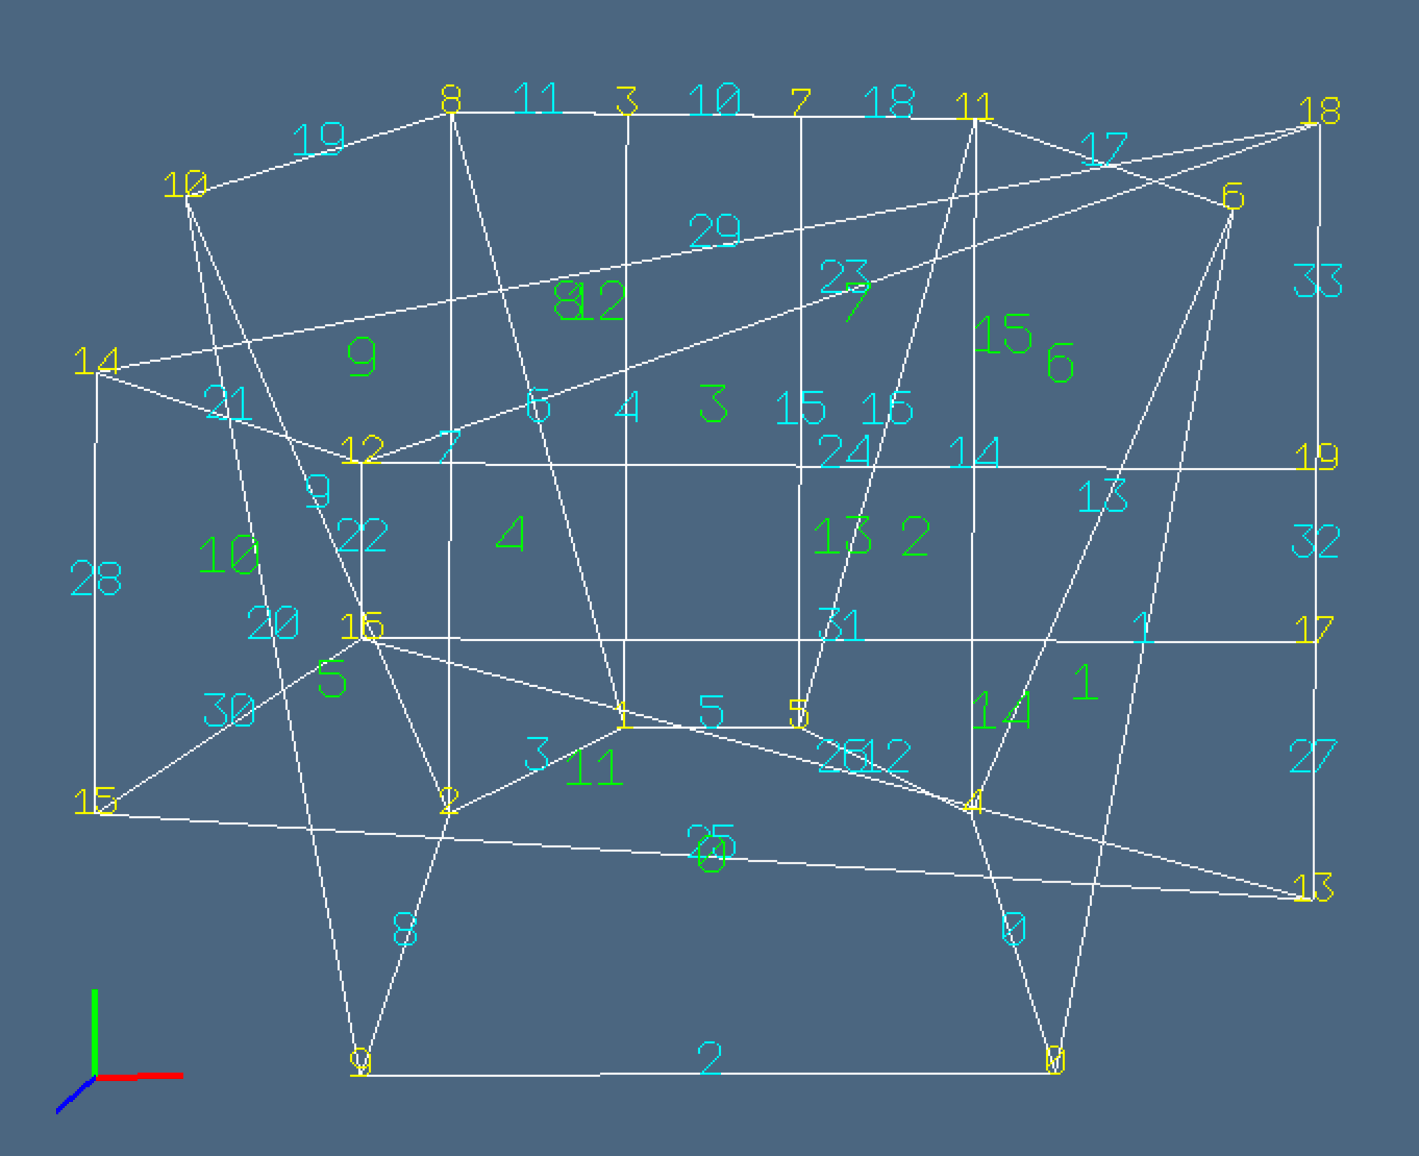
\includegraphics[width=0.6\linewidth]{images/covering} 
   \caption{Set covering of the two Boolean arguments.}
   \label{fig:example}
\end{figure}

\paragraph{Building a partition of common convex hull}

%-------------------------------------------------------------------------------
@D Building a partition of common convex hull of vertices
@{def partition(V, CV1,CV2, EEV1,EEV2):
	CV = sorted(AA(sorted)(Delaunay(array(V)).vertices))
	BV1, BV2, BF1, BF2 = boundaryVertices( V, CV1,CV2, 'cuboid', EEV1,EEV2 )
	BV = BV1+BV2
	nE1 = len(EEV1)
	BF = BF1+[e+nE1 for e in BF2]
	return CV, BV1, BV2, BF1, BF2, BV, BF, nE1
@}
%-------------------------------------------------------------------------------




\section{Selecting cells to split}


\paragraph{Relational inversion (Characteristic matrix transposition)}

%-------------------------------------------------------------------------------
@D Characteristic matrix transposition
@{""" Characteristic matrix transposition """
def invertRelation(V,CV):
	VC = [[] for k in range(len(V))]
	for k,cell in enumerate(CV):
		for v in cell:
			VC[v] += [k]
	return VC
@}
%-------------------------------------------------------------------------------


%-------------------------------------------------------------------------------
@D Look for cells in Delaunay, with vertices in both operands
@{""" Look for cells in Delaunay, with vertices in both operands """
def mixedCells(CV,CV1,CV2,n12):
	n0,n1 = 0, max(AA(max)(CV1))			# vertices in CV1 (extremes included)
	m0,m1 = n1+1-n12, max(AA(max)(CV2))		# vertices in CV2 (extremes included)
	return [list(cell) for cell in CV if any([ n0<=v<=n1 for v in cell]) 
		and any([ m0<=v<=m1 for v in cell])]
@}
%-------------------------------------------------------------------------------

%-------------------------------------------------------------------------------
@D Look for cells in cells12, with vertices on boundaries
@{""" Look for cells in cells12, with vertices on boundaries """
def mixedCellsOnBoundaries(cells12,BV):
	cells12BV = [cell for cell in cells12
					if len(list(set(cell).intersection(BV))) != 0]
	return cells12BV
@}
%-------------------------------------------------------------------------------

%-------------------------------------------------------------------------------
@D Build intersection tasks
@{""" Build intersection tasks """
def cuttingTest(cuttingHyperplane,polytope,V):
	signs = [INNERPROD([cuttingHyperplane, V[v]+[1.]]) for v in polytope]
	signs = eval(vcode(signs))
	return any([value<-0.001 for value in signs]) and any([value>0.001 for value in signs])

def splittingTasks(V,pivots,BV,BC,VBC,CV,VC):
	tasks = []
	for pivotCell in pivots:
		cutVerts = [v for v in pivotCell if v in BV]
		for v in cutVerts:
			cutFacets = VBC[v]
			cells2cut = VC[v]
			for face,cell in CART([cutFacets,cells2cut]):
				polytope = CV[cell]
				points = [V[w] for w in BC[face]]
				dim = len(points[0])
				theMat = Matrix( [(dim+1)*[1.]] + [p+[1.] for p in points] )
				cuttingHyperplane = [(-1)**(col)*theMat.minor(0,col).determinant() 
									for col in range(dim+1)]
				if cuttingTest(cuttingHyperplane,polytope,V):
					tasks += [[face,cell,cuttingHyperplane]]
	tasks = AA(eval)(set(AA(str)(tasks)))
	tasks = TrivialIntersection(tasks,V,BC,CV)
	return tasks
@}
%-------------------------------------------------------------------------------

\paragraph{facet-cell trivial intersection filtering}

A final filtering is applied to the pairs \texttt{(cutting\-Hyper\-plane,polytope} in the \texttt{tasks} array, in order to remove those facets (pairs in 2D) whose intersection reduces to a single point, i.e.~to the comman vertex between the boundary $(d-1)$-face, having \texttt{cuttingHyperplane} as affine hull, and the \texttt{polytope} $d$-cell.

For this purpose, it is checked that at least one of the facet vertices, transformed into the common-vertex-based coordinate frame, have all positive coordinates. This fact guarantees the existence of a non trivial intersection between the $(d-1)$-face and the $d$-cell.

%-------------------------------------------------------------------------------
@D Trivial intersection filtering
@{""" Trivial intersection filtering """
def TrivialIntersection(tasks,V,EEV,CV):
	out = []
	for face,cell,affineHull in tasks:
		faceVerts, cellVerts = EEV[face], CV[cell]
		v0 = list(set(faceVerts).intersection(cellVerts))[0] # v0 = common vertex
		transformMat = mat([VECTDIFF([V[v],V[v0]]) for v in cellVerts if v != v0]).T.I
		vects = (transformMat * (mat([VECTDIFF([V[v],V[v0]]) for v in faceVerts 
					if v != v0]).T)).T.tolist()
		if any([all([x>0 for x in list(vect)]) for vect in vects]): 
			out += [[face,cell,affineHull]]
	return out
@}
%-------------------------------------------------------------------------------


\section{Splitting cells traversing the boundaries}

In the previous section we computed a set of "slitting seeds", each made by a boundary facet and by a Delaunay cell to be splitted by the facet's affine hull. Here we show how to partition ate each such cells into two cells, according to Figure~\ref{fig:splitting}, where the boundary facets of the two boolean arguments are shown in yellow color.

\begin{figure}[htbp] %  figure placement: here, top, bottom, or page
   \centering
   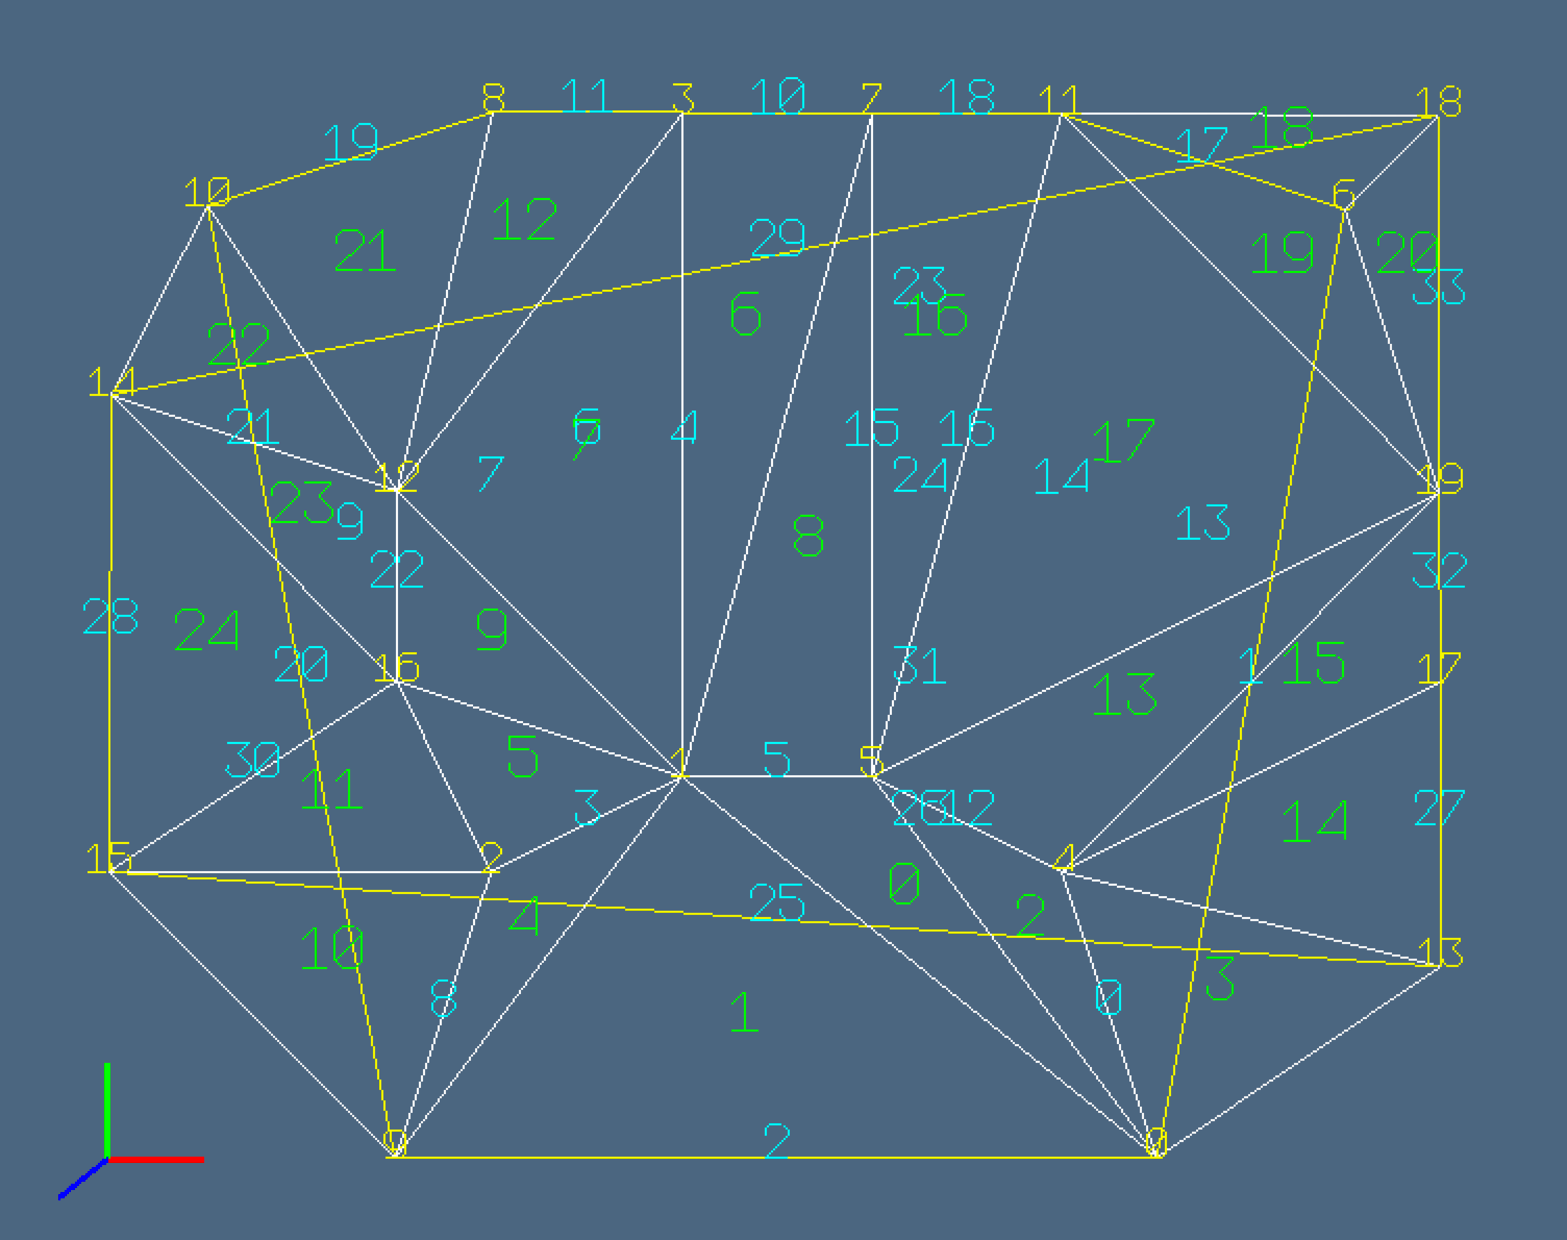
\includegraphics[width=0.6\linewidth]{images/splitting} 
   \caption{example caption}
   \label{fig:splitting}
\end{figure}

In the example in Figure~\ref{fig:splitting}, the set of pairs \texttt{(facet,cell)} to be used as splitting seeds are given below.
{\small
\begin{verbatim}
[[25, 3], [1, 3], [29, 18], [20, 22], [1, 19], [25, 10], [20, 10], [29, 22]]
\end{verbatim}}

\subsection{Cell splitting}

A cell will be split by pyplasm intersection with a suitable rotated and translated instance of a (large) $d$-cuboid with the superior face embedded in the hyperplane $z=0$.

\paragraph{Splitting a cell with an hyperplane}
The macro below defines a function \texttt{cellSplitting}, with input the index of the \texttt{face}, the index of the \texttt{cell} to be bisected, the \texttt{covector} giving the coefficients of the splitting hyperplane, i.e.~the affine hull of the splitting \texttt{face}, and the arrays \texttt{V}, \texttt{EEV}, \texttt{CV}, giving the coordinates of vertices, the (accumulated) facet to vertices relation (on the input models), and the cell to vertices relation (on the Delaunay model), respectively. 

The actual subdivision of the input \texttt{cell} onto the two output cells \texttt{cell1} and \texttt{cell2} is performed by using the \texttt{pyplasm} Boolean operations of intersection and difference of the input with a solid simulation of the needed hyperspace, provided by the \texttt{rototranslSubspace} variable. Of course, such pyplasm operators return two Hpc values, whose vertices will then extracted using the \texttt{UKPOL} primitive.

%-------------------------------------------------------------------------------
@D Cell splitting
@{""" Cell splitting in two cells """
def cellSplitting(face,cell,covector,V,EEV,CV):

	dim = len(V[0])
	subspace = (T(range(1,dim+1))(dim*[-50])(CUBOID(dim*[100])))
	normal = covector[:-1]
	if len(normal) == 2:  # 2D complex
		rotatedSubspace = R([1,2])(ATAN2(normal)-PI/2)(T(2)(-50)(subspace))
	elif len(normal) == 3:  # 3D complex
		rotatedSubspace = R()()(subspace)
	else: print "rotation error"
	t = V[EEV[face][0]]
	rototranslSubspace = T(range(1,dim+1))(t)(rotatedSubspace)
	cellHpc = MKPOL([V,[[v+1 for v in CV[cell]]],None])
	
	# cell1 = INTERSECTION([cellHpc,rototranslSubspace])
	tolerance=0.0001
	use_octree=False
	cell1 = Plasm.boolop(BOOL_CODE_AND, 
		[cellHpc,rototranslSubspace],tolerance,plasm_config.maxnumtry(),use_octree)
	verts,cells,pols = UKPOL(cell1)
	cell1 = AA(vcode)(verts)

	# cell2 = DIFFERENCE([cellHpc,rototranslSubspace])	
	cell2 = Plasm.boolop(BOOL_CODE_DIFF, 
		[cellHpc,rototranslSubspace],tolerance,plasm_config.maxnumtry(),use_octree)
	verts,cells,pols = UKPOL(cell2)
	cell2 = AA(vcode)(verts)

	return cell1,cell2
@}
%-------------------------------------------------------------------------------

\begin{figure}[htbp] %  figure placement: here, top, bottom, or page
   \centering
   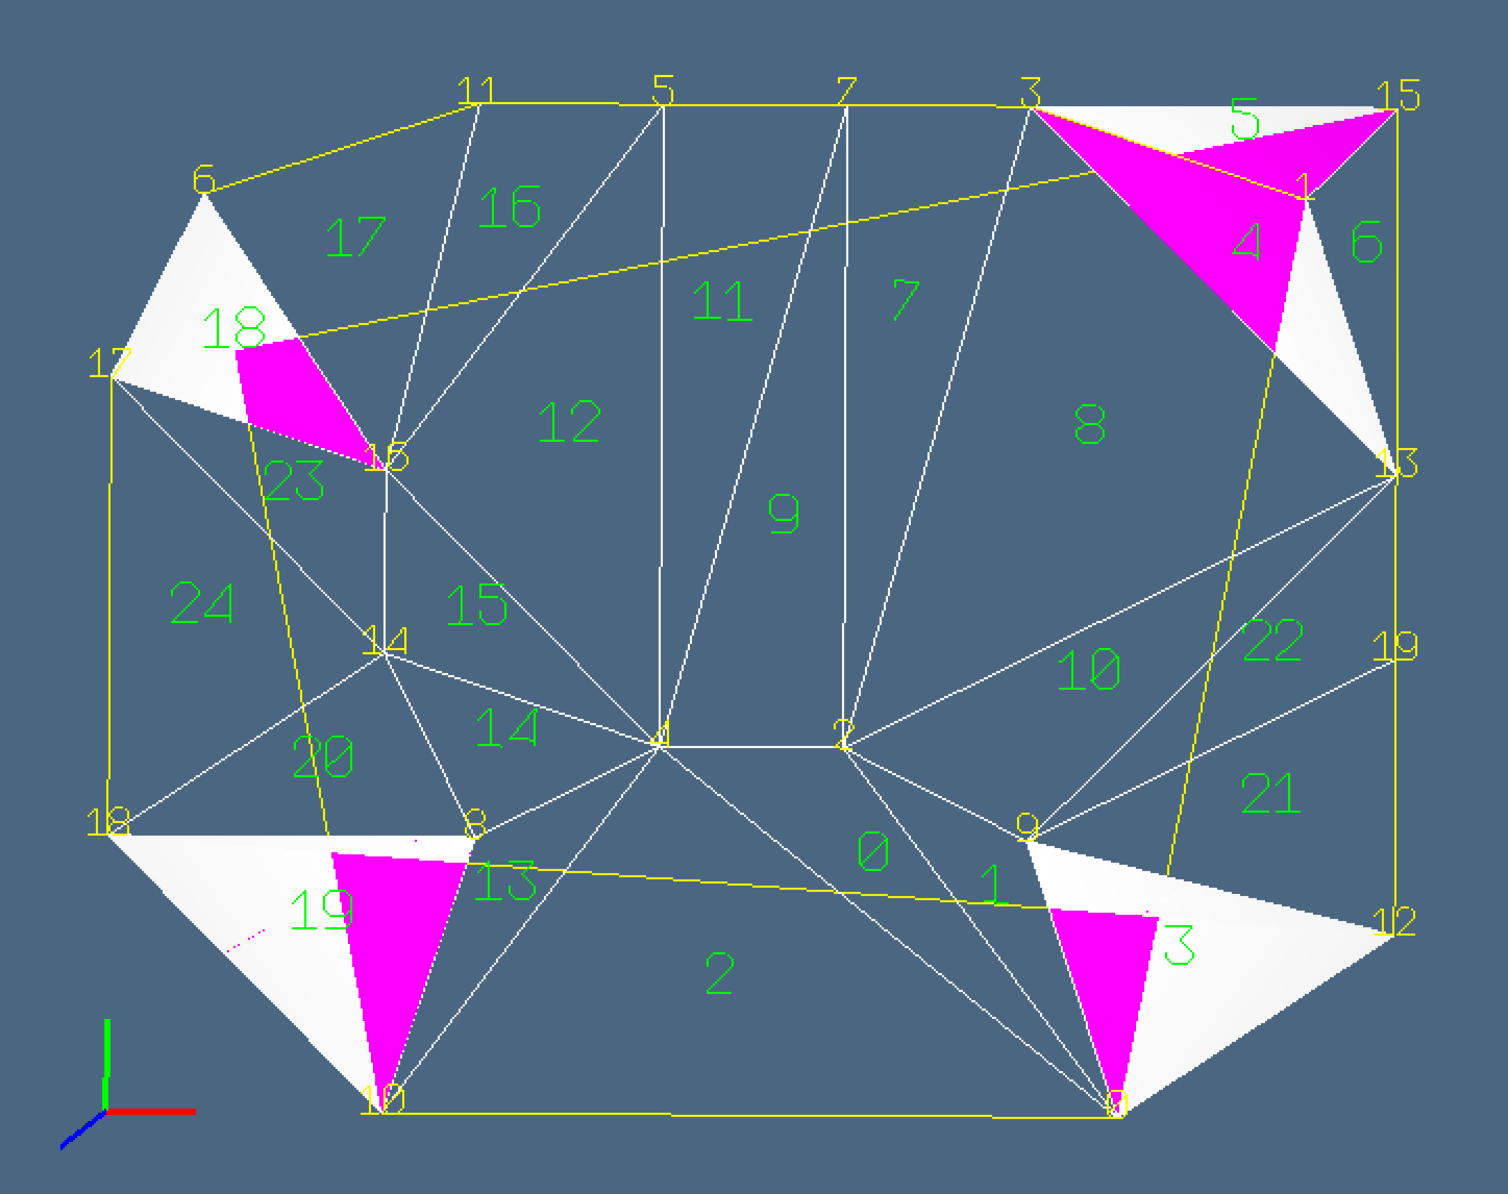
\includegraphics[width=0.6\linewidth]{images/seeds} 
   \caption{example caption}
   \label{fig:example}
\end{figure}


\subsection{Cross-building of two task dictionaries}

The correct and efficient splitting of the combined Delaunay complex (CDC) with the  (closed and orientable) boundaries of two Boolean arguments, requires the use of two special dictionaries, respectively named \texttt{dict\_fc} (for \emph{face-cell}), and \texttt{dict\_cf} (for \emph{cell-face}).
 
On one side, for each splitting facet ($(d-1)$-face), used as key, we store in \texttt{dict\_fc} the list of traversed $d$-cells of CDC, starting in 2D with the two cells containing the two extreme vertices of the cutting edge, and in higher dimensions, with all the $d$-cells containing one of vertices of the splitting $(d-1)$-face.

On the other side, for each $d$-cell to be split, used as key, we store in \texttt{dict\_cf} the list of cutting $(d-1)$-cells, since a single $d$-cell may be traversed and split by more than one facet. 


\paragraph{Init face-cell and cell-face dictionaries}

%-------------------------------------------------------------------------------
@D Init face-cell and cell-face dictionaries
@{""" Init face-cell and cell-face dictionaries """
def initTasks(tasks):
	dict_fc = defaultdict(list)
	dict_cf = defaultdict(list)
	for task in tasks:
		face,cell,covector = task
		dict_fc[face] += [(cell,covector)] 
		dict_cf[cell] += [(face,covector)] 
	return dict_fc,dict_cf
@}
%-------------------------------------------------------------------------------

\paragraph{Example of face-cell and cell-face dictionaries}

%-------------------------------------------------------------------------------
@D Example of face-cell and cell-face dictionaries
@{""" Example of face-cell and cell-face dictionaries """
tasks (face,cell) = [
 [0, 4, [-10.0, 2.0, 110.0]],
 [31, 5, [3.0, -14.0, 112.0]],
 [17, 18, [10.0, 2.0, -30.0]],
 [22, 3, [-1.0, -14.0, 42.0]],
 [17, 19, [10.0, 2.0, -30.0]],
 [31, 18, [3.0, -14.0, 112.0]],
 [22, 19, [-1.0, -14.0, 42.0]],
 [0, 3, [-10.0, 2.0, 110.0]]]

tasks (dict_fc) = defaultdict(<type 'list'>, {
  0: [(4, [-10.0, 2.0, 110.0]), (3, [-10.0, 2.0, 110.0])],
 17: [(18, [10.0, 2.0, -30.0]), (19, [10.0, 2.0, -30.0])],
 22: [(3, [-1.0, -14.0, 42.0]), (19, [-1.0, -14.0, 42.0])],
 31: [(5, [3.0, -14.0, 112.0]), (18, [3.0, -14.0, 112.0])]  })

tasks (dict_cf) = defaultdict(<type 'list'>, {
 19: [(17, [10.0, 2.0, -30.0]), (22, [-1.0, -14.0, 42.0])],
 18: [(17, [10.0, 2.0, -30.0]), (31, [3.0, -14.0, 112.0])],
  3: [(22, [-1.0, -14.0, 42.0]), (0, [-10.0, 2.0, 110.0])],
  4: [(0, [-10.0, 2.0, 110.0])],
  5: [(31, [3.0, -14.0, 112.0])]  })
@}
%-------------------------------------------------------------------------------


\subsection{Updating the vertex set and dictionary}

In any dimension, the split of a $d$-cell with an hyperplane (crossing its interior) produces two $d$-cells and some new vertices living upon the splitting hyperplane.

When the $d$-cell $c$ is contained in only one seed of the CDC decomposition, i.e.~when \texttt{dict\_cf[c]} has cardinality one (in other words: it is crossed only by one boundary facet), the two generated cells \texttt{vcell1,vcell2} can be safely output, and accommodated in two slots of the \texttt{CV} list.

Conversely, when more than one facet crosses $c$, much more care must be taken to guarantee the correct fragmentation of this cell.


\paragraph{Managing the splitting dictionaries}
The function \texttt{splittingControl} takes care of cells that must be split several times, as crossed by several boundary faces. 

If the dictionary item \texttt{dict\_cf[cell]} has \emph{length} one (i.e.~is crossed  \emph{only} by one face) the \texttt{CV} list is updated and the function returns, in order to update the \texttt{dict\_fc} dictionary.

Otherwise, the function subdivides the facets cutting \texttt{cell} between those to be associated to \texttt{vcell1} and to \texttt{vcell2}. 
For each pair \texttt{aface,covector} in \texttt{dict\_cf[cell]} \emph{and} in position following \texttt{face} in the list of pairs, check if either \texttt{vcell1} or \texttt{vcell2} or both, have intersection with the subset of vertices shared between \texttt{cell} and \texttt{aface}, and respectively put in \texttt{alist1}, in \texttt{alist2}, or in both.
Finally, store \texttt{vcell1} and \texttt{vcell2} in \texttt{CV}, and \texttt{alist1}, \texttt{alist2} in \texttt{dict\_cf}.

TODO: update \texttt{dict\_fc} ...

%-------------------------------------------------------------------------------
@D Managing the splitting dictionaries
@{""" Managing the splitting dictionaries """
def splittingControl(face,cell,covector,vcell1,vcell2,dict_fc,dict_cf,V,BC,CV,VC):

   print "vcell1,vcell2 =",vcell1,vcell2
   # only one facet covector crossing the cell
   cellVerts = CV[cell]
   CV[cell] = vcell1
   CV += [vcell2]
   print "covector =",covector
   dict_fc[face].remove((cell,covector))   # remove the split cell
   dict_cf[cell].remove((face,covector))   # remove the splitting face
         
   # more than one facet covectors crossing the cell
   alist1,alist2 = list(),list()
   for aface,covector in dict_cf[cell]:
   
      # for each facet crossing the cell
      # compute the intersection between the facet and the cell
      faceVerts = BC[aface]
      commonVerts = list(set(faceVerts).intersection(cellVerts))
      
      # and attribute the intersection to the split subcells
      if set(vcell1).intersection(commonVerts) != set():
         alist1.append((aface,covector))
      else: dict_fc[aface].remove((cell,covector)) 
            
      if set(vcell2).intersection(commonVerts) != set():
         alist2.append((aface,covector))
         dict_fc[aface] += [(len(CV)-1,covector)]
   
   dict_cf[cell] = alist1  
   dict_cf[len(CV)-1] = alist2
   return V,CV, dict_cf, dict_fc
@}
%-------------------------------------------------------------------------------


\paragraph{Updating the vertex set of split cells}
The code in the macro below provides the splitting of the CDC along the boundaries of the two Boolean arguments.
This function, and the ones called by its, provide the dynamic update of the two main data structures, i.e.~of the LAR model \texttt{(V,CV)}.

%-------------------------------------------------------------------------------
@D Updating the vertex set  of split cells
@{""" Updating the vertex set of split cells """
def splitCellsCreateVertices(vertdict,dict_fc,dict_cf,V,BC,CV,VC):
	DEBUG = False
	nverts = len(V); cellPairs = []
	while any([tasks != [] for face,tasks in dict_fc.items()]) : 
		for face,tasks in dict_fc.items():
			for task in tasks:
				cell,covector = task
				if cuttingTest(covector,CV[cell],V):
					cell1,cell2 = cellSplitting(face,cell,covector,V,BC,CV)
					if cell1 == [] or cell2 == []:
						print "\nface,cell,covector =",face,cell,covector
						print "cell1,cell2 =",cell1,cell2
					else:
						adjCells = adjacencyQuery(V,CV)(cell)
						vcell1 = []
						for k in cell1:
							if vertdict[k]==[]: 
								vertdict[k] += [nverts]
								V += [eval(k)]
								nverts += 1
							vcell1 += [vertdict[k]]
						
						vcell1 = CAT(vcell1)
						vcell2 = CAT([vertdict[k] for k in cell2])						
						V,CV, dict_cf, dict_fc = splittingControl(face,cell,covector,vcell1,vcell2, 
														dict_fc,dict_cf,V,BC,CV,VC)
						for adjCell in adjCells:
							if cuttingTest(covector,CV[adjCell],V) and not ((face,covector) in dict_cf[adjCell]):
								dict_fc[face] += [(adjCell,covector)] 
								dict_cf[adjCell] += [(face,covector)] 
						cellPairs += [[vcell1, vcell2]]
					if DEBUG: showSplitting(V,cellPairs,BC,CV)
				else:
					dict_fc[face].remove((cell,covector))   # remove the split cell
					dict_cf[cell].remove((face,covector))   # remove the splitting face
	return cellPairs
@}
%-------------------------------------------------------------------------------


\subsection{Updating the split cell and the stack of seeds}

When a $d$-cell of the combined Delaunay complex (CDC) is split into two $d$-cells, the first task to perform is to update its representation as vertex list, and to update the list of $d$-cells. In particular, as \texttt{cell}, and \texttt{cell1}, \texttt{cell2} are the input $d$-cell and the two output $d$-cells, respectively, we go to substitute \texttt{cell} with \texttt{cell1}, and to add the \texttt{cell2} as a new row of the \texttt{CSR}$(M_d)$ matrix, i.e.~as the new terminal element of the \texttt{CV} array. Of course, the reverse relation \texttt{VC} must be updated too.

\paragraph{Updating the split cell} 
First of all notice that, whereas \texttt{cell} is given as an integer index to a \texttt{CV} row,
\texttt{cell1}, \texttt{cell2} are returned by the \texttt{cellSplitting} function as lists of lists of coordinates (of vertices). Therefore such vectors must be suitably transformed into dictionary keys, in order to return the corresponding vertex indices. When transformed into two lists of vector indices, \texttt{cell1}, \texttt{cell2} will be in the form needed to update the \texttt{CV} and \texttt{VC} relations.

%-------------------------------------------------------------------------------
@D Updating the split cell
@{""" Updating the split cell """
def splitCellUpdate(cell,vcell1,vcell2,CV):
	newVerts = list(set(vcell1).difference(CV[cell]))
	return newVerts
@}
%-------------------------------------------------------------------------------



\subsection{Updating the cells adjacent to the split cell}

Once the list of $d$-cells has been updated with respect to the results of a split operation, it is necessary to consider the possible update of all the cells that are adjacent to the split one.  It particular we need to update their lists of vertices, by introducing the new vertices produced by the split, and by updating the dictionaries of tasks, by introducing the new (adjacent) splitting seeds.

\paragraph{Computing the adjacent cells of a given cell}
To perform this task we make only use of the \texttt{CV} list. In a more efficient implementation we should make direct use of the sparse adjacency matrix, to be dynamically updated together with the \texttt{CV} list.
The computation of the adjacent $d$-cells of a single $d$-cell is given here by extracting a column of the $\texttt{CSR}(M_d\, M_d^t)$. This can be done by multiplying $\texttt{CSR}(M_d)$ by its transposed row corresponding to the query $d$-cell. 

%-------------------------------------------------------------------------------
@D Computing the adjacent cells of a given cell
@{""" Computing the adjacent cells of a given cell """
def adjacencyQuery (V,CV):
	dim = len(V[0])
	def adjacencyQuery0 (cell):
		nverts = len(CV[cell])
		csrCV =  csrCreate(CV)
		csrAdj = matrixProduct(csrCV,csrTranspose(csrCV))
		cellAdjacencies = csrAdj.indices[csrAdj.indptr[cell]:csrAdj.indptr[cell+1]]
		return [acell for acell in cellAdjacencies if dim <= csrAdj[cell,acell] < nverts]
	return adjacencyQuery0
@}
%-------------------------------------------------------------------------------

\paragraph{Updating the adjacency matrix}
At every step of the CDC splitting, generating two output cells \texttt{cell1} and  \texttt{cell2} from the input  \texttt{cell}, the element of such index in the list \texttt{CV} is restored with the \texttt{cell1} vertices, and a new (last) element is created in \texttt{CV}, to store the \texttt{cell2} vertices.
Therefore the row of index \texttt{cell} of the symmetric  adjacency matrix must be recomputed, being the \texttt{cell} column updated consequently. Also, a new last row (and column) must be added to the matrix. 

%-------------------------------------------------------------------------------
@D Updating the adjacency matrix
@{""" Updating the adjacency matrix """
pass
@}
%-------------------------------------------------------------------------------


\section{Reconstruction of results}


\subsection{The Boolean algorithm flow}


\paragraph{The splitting of Common Delaunay Complex}

%-------------------------------------------------------------------------------
@D Splitting the Common Delaunay Complex
@{""" Splitting of Common Delaunay Complex """
def booleanBulk(V,n12,EEV,CV,VC,BF,CV1,CV2,EEV1,EEV2,BV,BV1,BV2,VEE1,VEE2):
	VE = [VEE1[v]+VEE2[v] for v in range(len(V))]
	cells12 = mixedCells(CV,CV1,CV2,n12)
	pivots = mixedCellsOnBoundaries(cells12,BV1,BV2)
	tasks = splittingTasks(V,pivots,BV,BF,VC,CV,EEV,VE)
		
	dict_fc,dict_cf = initTasks(tasks)
	vertdict = defaultdict(list)
	for k,v in enumerate(V): vertdict[vcode(v)] += [k]
	cellPairs = splitCellsCreateVertices(vertdict,dict_fc,dict_cf,V,EEV,CV,VC,BF)
	return cellPairs
@}
%-------------------------------------------------------------------------------

\paragraph{Show the process of CDC splitting}

%-------------------------------------------------------------------------------
@D Show the process of CDC splitting
@{""" Show the process of CDC splitting """
def showSplitting(V,cellPairs,BC,CV):
	VV = AA(LIST)(range(len(V)))
	boundaries = COLOR(RED)(SKEL_1(STRUCT(MKPOLS((V,BC)))))
	submodel = COLOR(CYAN)(STRUCT([ SKEL_1(STRUCT(MKPOLS((V,CV)))), boundaries ]))
	if cellPairs != []:
		cells1,cells2 = TRANS(cellPairs)
		out = [COLOR(WHITE)(MKPOL([V,[[v+1 for v in cell] for cell in cells1],None])), 
				COLOR(MAGENTA)(MKPOL([V,[[v+1 for v in cell] for cell in cells2],None]))]
		VIEW(STRUCT([ STRUCT(out),larModelNumbering(V,[VV,BC,CV],submodel,2) ]))
	else:
		VIEW(STRUCT([ larModelNumbering(V,[VV,BC,CV],submodel,2) ]))
@}
%-------------------------------------------------------------------------------



\section{Exporting the library}


%-------------------------------------------------------------------------------
@O lib/py/bool.py
@{""" Module for Boolean ops with LAR """
from matrix import *
@< Initial import of modules @>
@< Symbolic utility to represent points as strings @>
@< Place the vertices of Boolean arguments in a common space @>
@< Building a covering of common convex hull @>
@< Building a partition of common convex hull of vertices @>
@< Characteristic matrix transposition @>
@< Look for cells in Delaunay, with vertices in both operands @>
@< Look for cells in cells12, with vertices on boundaries @>
@< Build intersection tasks @>
@< Trivial intersection filtering @>
@< Cell splitting @>
@< Init face-cell and cell-face dictionaries @>
@< Updating the split cell @>
@< Updating the vertex set  of split cells @>
@< Managing the splitting dictionaries @>
@< Computing the adjacent cells of a given cell @>
@< Splitting the Common Delaunay Complex @>
@< Show the process of CDC splitting @>
@}
%-------------------------------------------------------------------------------

\section{Tests}



\subsection{2D examples}

\subsubsection{First examples}

Three sets of input 2D data are prepared here, ranging from very simple to a small instance of the hardest kind of dataset, known to produce an output of size $O(n^2)$.


%-------------------------------------------------------------------------------
@D First set of 2D data: Fork-0 input
@{""" Definition of Boolean arguments """
V1 = [[3,0],[11,0], [13,10], [10,11], [8,11], [6,11], [4,11], [1,10], [4,3], [6,4], 
	[8,4], [10,3]]
FV1 = [[0,1,8,9,10,11],[1,2,11], [3,10,11], [4,5,9,10], [6,8,9], [0,7,8], [2,3,11],
	[3,4,10], [5,6,9], [6,7,8]]
EV1 = [[0,1],[0,7],[0,8],[1,2],[1,11],[2,3],[2,11],[3,4],[3,10],[3,11],[4,5],[4,10],[5,6],[5,9],[6,7],[6,8],[6,9],[7,8],[8,9],[9,10],[10,11]]
VV1 = AA(LIST)(range(len(V1)))

V2 = [[0,3],[14,2], [14,5], [14,7], [14,11], [0,8], [3,7], [3,5]]
FV2 =[[0,5,6,7], [0,1,7], [4,5,6], [2,3,6,7], [1,2,7], [3,4,6]]
EV2 = [[0,1],[0,5],[0,7],[1,2],[1,7],[2,3],[2,7],[3,4],[3,6],[4,5],[4,6],[5,6],[6,7]]
VV2 = AA(LIST)(range(len(V2)))
@}
%-------------------------------------------------------------------------------


\paragraph{Input and visualisation of Boolean arguments}

%-------------------------------------------------------------------------------
@D Computation of lower-dimensional cells
@{""" Computation of edges an input visualisation """
model1 = V1,FV1
model2 = V2,FV2
basis1 = [VV1,EV1,FV1]
basis2 = [VV2,EV2,FV2]
submodel12 = STRUCT(MKPOLS((V1,EV1))+MKPOLS((V2,basis2[1])))
VIEW(larModelNumbering(V1,basis1,submodel12,4))
VIEW(larModelNumbering(V2,basis2,submodel12,4))
@}
%-------------------------------------------------------------------------------

\paragraph{Exporting test file}

%-------------------------------------------------------------------------------
@D Bulk of Boolean task computation
@{""" Bulk of Boolean task computation """
@< Computation of lower-dimensional cells @>

V,[VV,_,_,CV1,CV2],n12 = covering(model1,model2,2,0)
CV = sorted(AA(sorted)(Delaunay(array(V)).vertices))
vertdict = defaultdict(list)
for k,v in enumerate(V): vertdict[vcode(v)] += [k]

BC1 = boundaryCells(basis1[-1],basis1[-2])
BC2 = boundaryCells(basis2[-1],basis2[-2])
BC = [[ vertdict[vcode(V1[v])][0] for v in basis1[-2][cell]] for cell in BC1] + [ [ vertdict[vcode(V2[v])][0] for v in basis2[-2][cell]] for cell in BC2]
BC = sorted(AA(sorted)(BC))

BV1 = list(set(CAT([basis1[-2][bc] for bc in BC1])))
BV1 = [vertdict[vcode(V1[v])][0] for v in BV1]
BV2 = list(set(CAT([basis2[-2][bc] for bc in BC2])))
BV1 = [vertdict[vcode(V2[v])][0] for v in BV2]
BV = list(set(CAT([v for v in BC])))
VV = AA(LIST)(range(len(V)))
submodel = STRUCT([SKEL_1(STRUCT(MKPOLS((V,CV)))), COLOR(RED)(STRUCT(MKPOLS((V,BC))))])
VIEW(larModelNumbering(V,[VV,BC,CV],submodel,4))

cells12 = mixedCells(CV,CV1,CV2,n12)
pivots = mixedCellsOnBoundaries(cells12,BV)
VBC = invertRelation(V,BC)
VC = invertRelation(V,CV)
tasks = splittingTasks(V,pivots,BV,BC,VBC,CV,VC)
dict_fc,dict_cf = initTasks(tasks)

cellPairs = splitCellsCreateVertices(vertdict,dict_fc,dict_cf,V,BC,CV,VC)
showSplitting(V,cellPairs,BC,CV)
@}
%-------------------------------------------------------------------------------


%-------------------------------------------------------------------------------
@O test/py/bool/test01.py
@{import sys
""" import modules from larcc/lib """
sys.path.insert(0, 'lib/py/')
from bool import *
@< First set of 2D data: Fork-0 input @>
@< Bulk of Boolean task computation @>
@}
%-------------------------------------------------------------------------------


\subsubsection{Two squares}




%-------------------------------------------------------------------------------
@o test/py/bool/test03.py
@{""" import modules from larcc/lib """
import sys
sys.path.insert(0, 'lib/py/')
from bool import *

V1 = [[0,0],[10,0],[10,10],[0,10]]
FV1 = [range(4)]
EV1 = [[0,1],[1,2],[2,3],[3,0]]
VV1 = AA(LIST)(range(len(V1)))

V2 = [[2.5,2.5],[12.5,2.5],[12.5,12.5],[2.5,12.5]]
FV2 = [range(4)]
EV2 = [[0,1],[1,2],[2,3],[3,0]]
VV2 = AA(LIST)(range(len(V2)))
@< Bulk of Boolean task computation @>
@}
%-------------------------------------------------------------------------------


%-------------------------------------------------------------------------------
@o test/py/bool/test04.py
@{""" import modules from larcc/lib """
import sys
sys.path.insert(0, 'lib/py/')
from bool import *

V1 = [[0,0],[10,0],[10,10],[0,10]]
FV1 = [range(4)]
EV1 = [[0,1],[1,2],[2,3],[3,0]]
VV1 = AA(LIST)(range(len(V1)))

V2 = [[2.5,2.5],[7.5,2.5],[7.5,7.5],[2.5,7.5]]
FV2 = [range(4)]
EV2 = [[0,1],[1,2],[2,3],[3,0]]
VV2 = AA(LIST)(range(len(V2)))
@< Bulk of Boolean task computation @>
@}
%-------------------------------------------------------------------------------


\begin{figure}[htbp] %  figure placement: here, top, bottom, or page
   \centering
   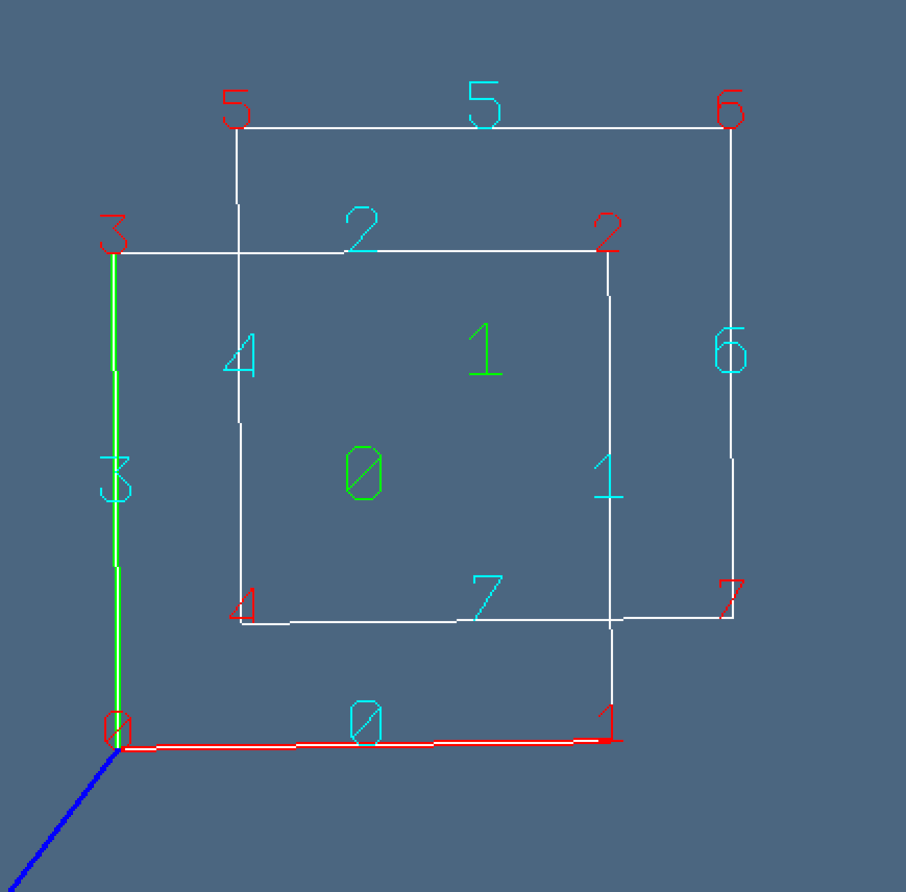
\includegraphics[height=0.244\linewidth,width=0.244\linewidth]{images/twosquares1} 
   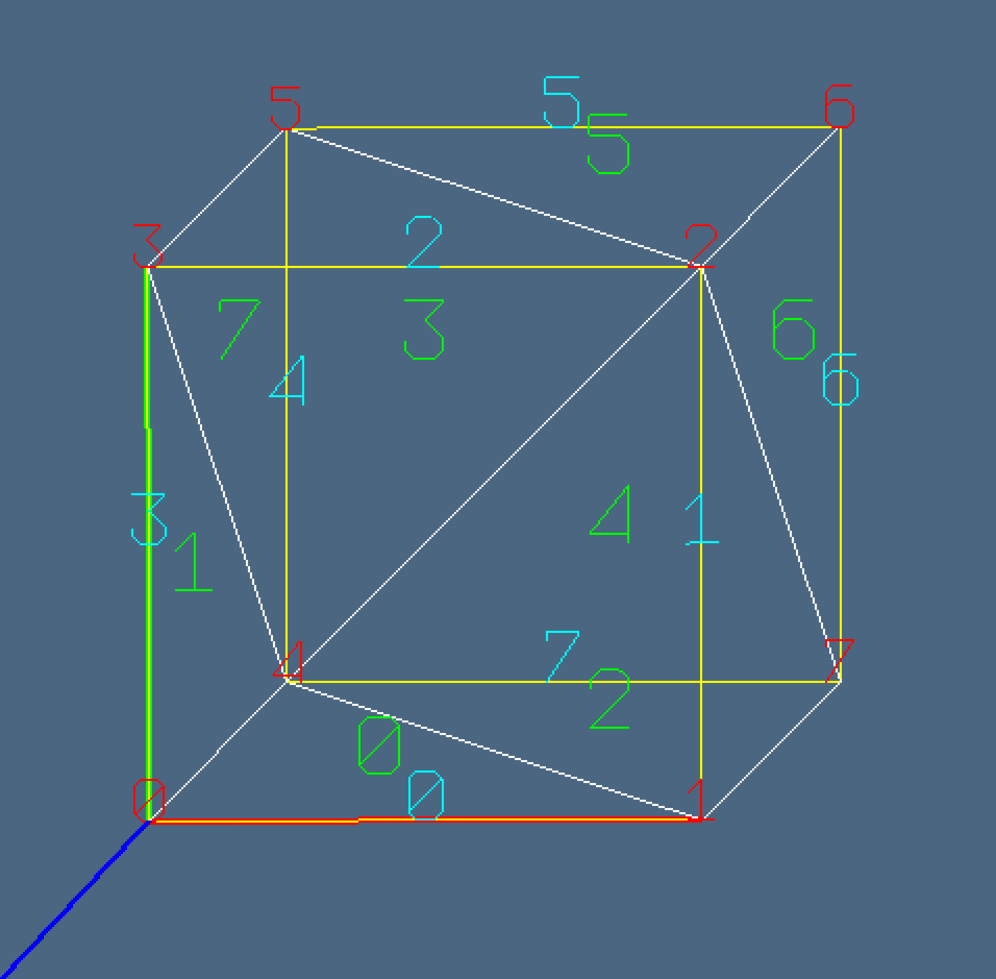
\includegraphics[height=0.244\linewidth,width=0.244\linewidth]{images/twosquares2} 
   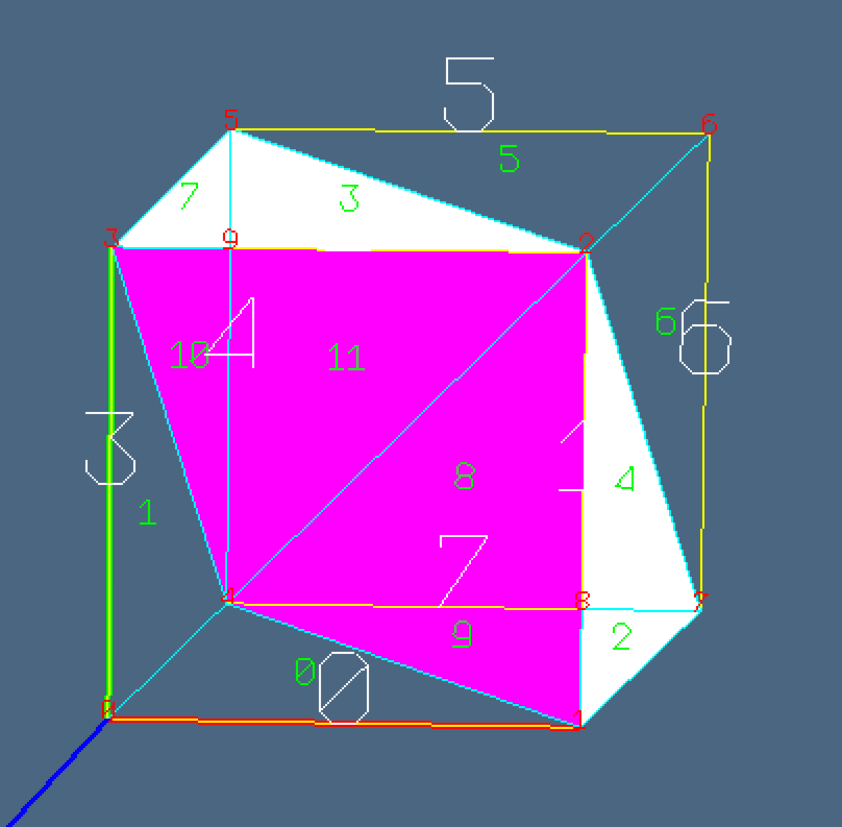
\includegraphics[height=0.244\linewidth,width=0.244\linewidth]{images/twosquares3} 
   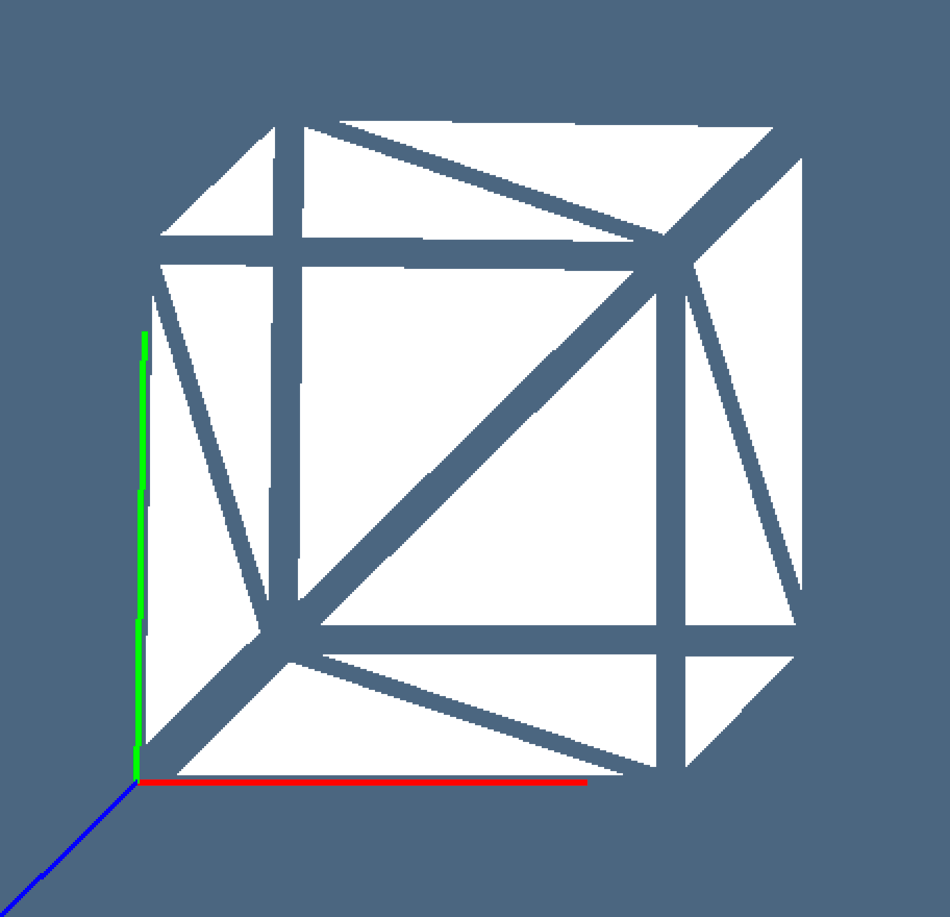
\includegraphics[height=0.244\linewidth,width=0.244\linewidth]{images/twosquares4} 
   \caption{Partitioning of the CDC (Common Delaunay Complex): (a) the two Boolean arguments merged in a single covering; (b) the CDC together with the two (yellow) boundaries; (c) the split CDC cells; (d) the exploded CDC partition.}
   \label{fig:example}
\end{figure}


%>>>>>>>>>>>>>>>>>>>>>>>>>>>>>>>>>>>>>>>>>>>>>>>>>>>>>>>>>>>>>>>>>>>>>>>>>>>>>>>
\appendix
%>>>>>>>>>>>>>>>>>>>>>>>>>>>>>>>>>>>>>>>>>>>>>>>>>>>>>>>>>>>>>>>>>>>>>>>>>>>>>>>
%-------------------------------------------------------------------------------
\section{Appendix: utility functions}
%-------------------------------------------------------------------------------
@D Initial import of modules
@{from pyplasm import *
from scipy import *
import sys
""" import modules from larcc/lib """
sys.path.insert(0, 'lib/py/')
from lar2psm import *
from simplexn import *
from larcc import *
from largrid import *
from myfont import *
from mapper import *
@}
%------------------------------------------------------------------
\subsection{Numeric utilities}

A small set of utilityy functions is used to transform a point representation as array of coordinates into a string of fixed format to be used as point key into python dictionaries.

%------------------------------------------------------------------
@D Symbolic utility to represent points as strings
@{""" TODO: use package Decimal (http://docs.python.org/2/library/decimal.html) """
PRECISION = 4 

def prepKey (args): return "["+", ".join(args)+"]"

def fixedPrec(value):
	out = round(value*10**PRECISION)/10**PRECISION
	if out == -0.0: out = 0.0
	return str(out)
	
def vcode (vect): 
	"""
	To generate a string representation of a number array.
	Used to generate the vertex keys in PointSet dictionary, and other similar operations.
	"""
	return prepKey(AA(fixedPrec)(vect))
@}
%------------------------------------------------------------------


\bibliographystyle{amsalpha}
\bibliography{bool}

\end{document}
